\chapter{Results}
\label{chp_res}


To evaluate the \textit{Hierarchical Temporal Memory} (HTM) model, described in the previous chapter, the HTM model is trained on the entire data set once, i.e. \textit{one-shot learning}. This was mainly because the data set was not split into a training and test set. The reason for this was due to the skewed distribution of the data set, see \autoref{table:dataset}, and the lack of shared vocabulary of system logs belonging to the same fault class.


The evaluation of the HTM model is divided into two to parts. First, we measure the performance of the HTM models predictions. Then, we compare them to the statistics collected from the Linnaeus model.


The predictions from the HTM model was obtained by doing inference on seen data, i.e. the entire data set. Three different inference experiments where carried out, where the first test was done with the system logs unaltered. The following two experiments inference was done on system logs with introduced errors. In the second test, ten per cent of the words in each system log were randomly dropped. And in the third test twenty per cent of all words in a sequence were dropped. We call these randomly introduced errors as \textit{``drop-out''} for the remainder of the thesis. These experiments aim to evaluate the robustness of the HTM model to changes in the system logs. The drop-outs represent what would happen if a developer rewrote a system log and changed some of the vocabulary, where some words are not in the GloVe matrix and can therefore not be encoded as SDRs.



\section{Evaluation of the Inference}
The evaluation will be presented in the following order; first, we present the confusion matrix to get an overview of the HTM models performance. Next, the recall of each fault class, to visualise the ability of the HTM model to find fault sequence of a specific fault class. Finally, we have the classification accuracy of each fault class. This gives us an indication of how well the HTM model is at classifying sequences correctly, and at the same time not classifying a sequence to a class it does not belong to.



\subsection{Inference on Unalterd System Logs}
In the first experiment inference was done on unaltered system logs. In \autoref{fig:confmatrix}, a comparison between the actual fault categories and the predictions made by the HTM model is visualised. A strong diagonal indicates that most predictions were \textit{True Positives}, i.e. the actual fault label. The \textit{unknown} class indicates sequences when the HTM model could not predict a fault label at all. From the confusion matrix, a observation can be made that the most of the misclassification belong to the \textit{nofault} class. There are two reasons why this type of misclassification happens, first, most of the system logs belongs to this class, see \autoref{table:dataset}. The second being that the the structure and the words occurring in the system logs are not different enough for the HTM model to distinguish them properly. In \autoref{fig:recall}, the recall of each class is presented, with \textit{com}, \textit{lm}, and \textit{sec} being most difficult to correctly classify. An important observation is that these classes has the fewest examples. The accuracy, see \autoref{fig:acc}, of the HTM model is high, but as stated before, this measure is saturated by the sheer number of \textit{nofaults}.

\clearpage

\begin{figure}[H]
    %\vspace{-8cm}
    \centering
    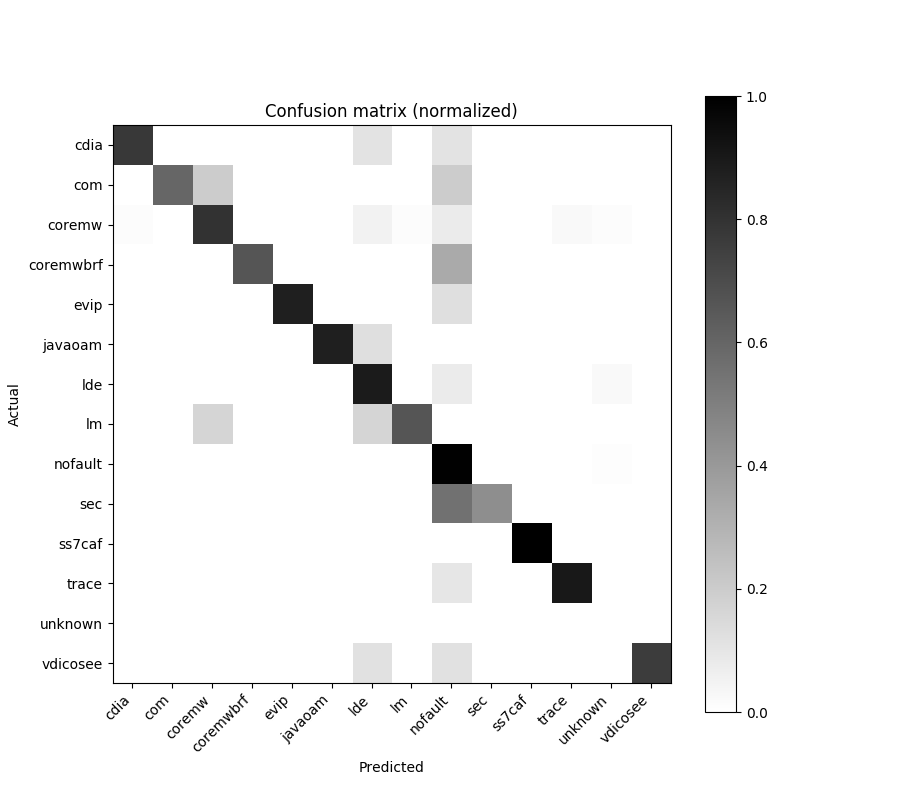
\includegraphics[width=\textwidth]{results/figures/256_32_0pcterror.png}
    \caption{The confusion matrix of the classification made by the HTM model with complete system logs. The vertical axis represent the actual sequence presented to the HTM model, and the horizontal axis represent the predicted fault class.}
    \label{fig:confmatrix}
\end{figure}



\begin{figure}[H]
  \centering
    \scalebox{.61}{    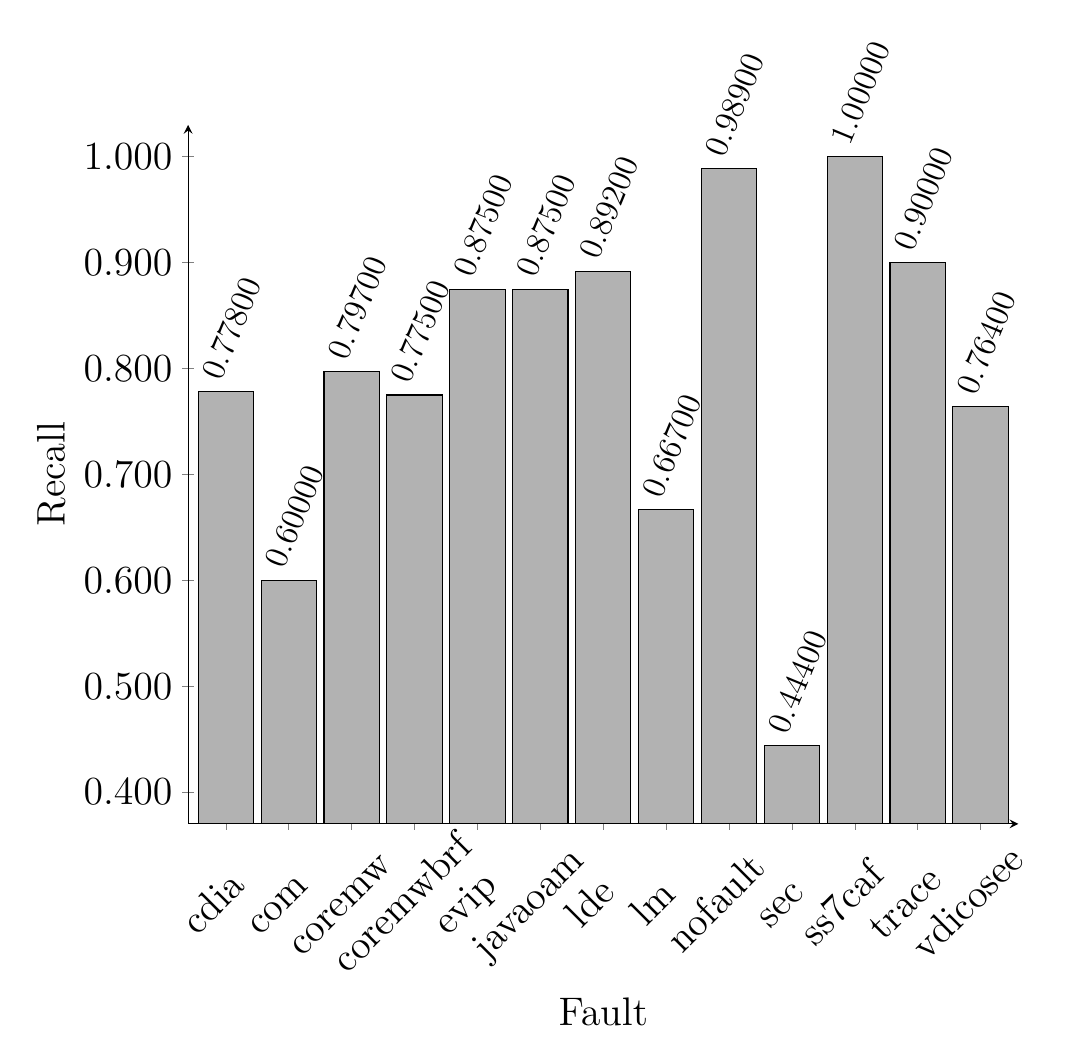
\begin{tikzpicture}[font=\Large]
    \begin{axis}[
      width=\textwidth,
      ybar,
      font=\Large,
      bar width=20pt,
      xlabel={Fault},
      ylabel={Recall},
      xticklabel style={rotate=45,anchor=base,yshift=-20,xshift=-22},
      xtick=data,
      ymin=0.400,
      ymax=1.00,
      axis x line=bottom,
      axis y line=left,
      enlarge x limits=0.1,
      enlargelimits=0.05,
      domain=0.40:1.000,
              y tick label style={
            /pgf/number format/.cd,
            fixed,
            zerofill,
            precision=3,
            /tikz/.cd,},
      symbolic x coords={cdia,com,coremw,coremwbrf,evip,javaoam,lde,lm,nofault,sec,ss7caf,trace,vdicosee},
      nodes near coords={\pgfmathprintnumber[fixed zerofill, precision=5]{\pgfplotspointmeta}},
      every node near coord/.append style={color=black, rotate=67.5, anchor=center, font=\large, xshift=22, yshift=7}],

    ]
      \addplot[fill=black!30] coordinates {
        (cdia,0.778) (com,0.6) 
		(coremw,.797) (coremwbrf,0.775) (evip,0.875) (javaoam, 0.875) (lde, 0.892) (lm, 0.667) (nofault,0.989) (sec, 0.444) (ss7caf, 1.0) (trace, 0.9) (vdicosee,0.764)
      };
    \end{axis}
  \end{tikzpicture}}
    \caption{Recall of each fault class with complete system logs presented to the HTM model.}
    \label{fig:recall}

    \vspace*{\floatsep}% https://tex.stackexchange.com/q/26521/5764

    \scalebox{.61}{    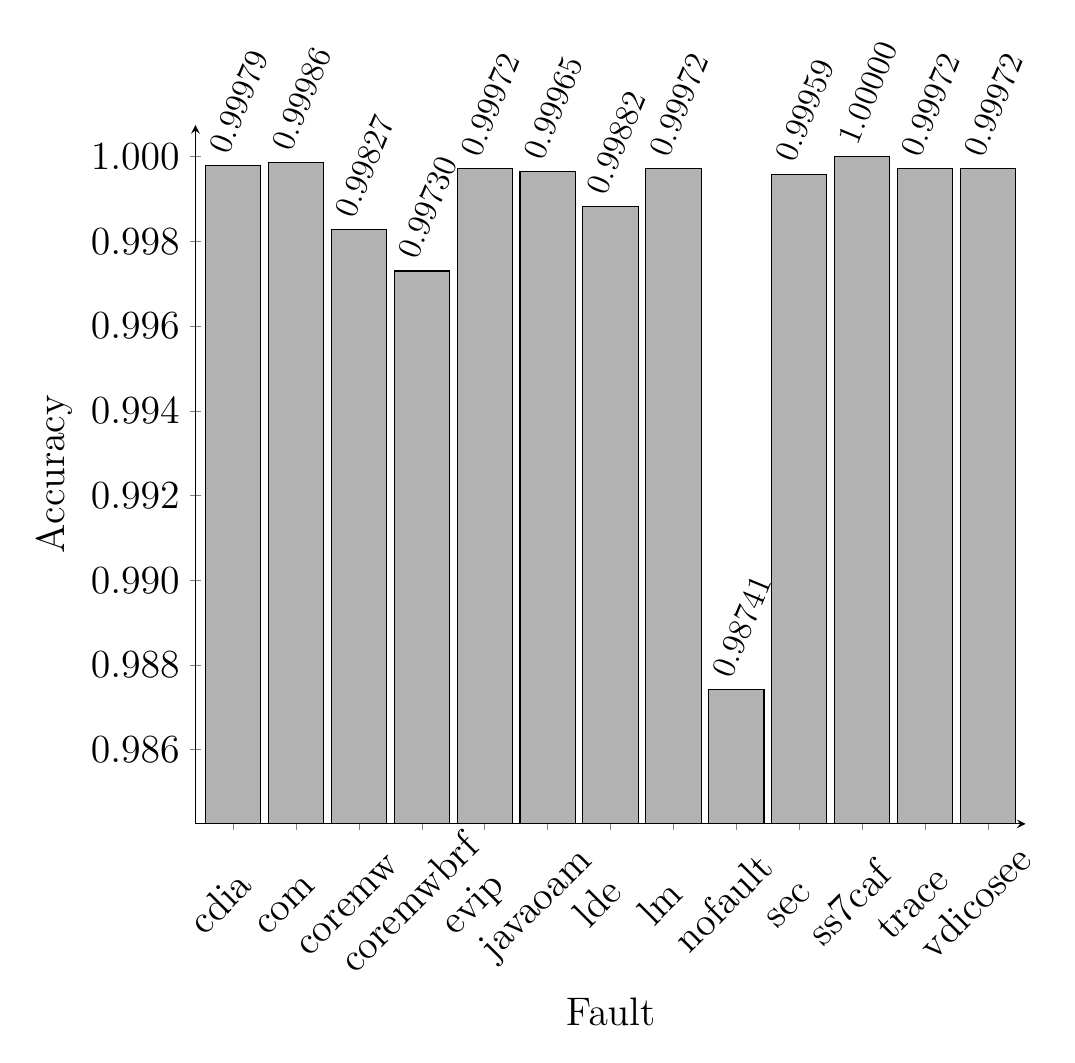
\begin{tikzpicture}[font=\Large]
    \begin{axis}[
      width=\textwidth,
      ybar,
      font=\Large,
      bar width=20pt,
      xlabel={Fault},
      ylabel={Accuracy},
      xticklabel style={rotate=45,anchor=base,yshift=-20,xshift=-22},
      xtick=data,
      ymin=0.985000,
      ymax=1.000000,
      axis x line=bottom,
      axis y line=left,
      enlarge x limits=0.1,
      enlargelimits=0.05,
      domain=0.98500:1.000000,
              y tick label style={
            /pgf/number format/.cd,
            fixed,
            zerofill,
            precision=3,
            /tikz/.cd,},
      symbolic x coords={cdia,com,coremw,coremwbrf,evip,javaoam,lde,lm,nofault,sec,ss7caf,trace,vdicosee},
      nodes near coords={\pgfmathprintnumber[fixed zerofill, precision=5]{\pgfplotspointmeta}},
      every node near coord/.append style={font=\large, color=black, rotate=67.5, anchor=center, xshift=22, yshift=7}],

    ]
      \addplot[fill=black!30] coordinates {
        (cdia,0.999793) (com,0.999862) 
		(coremw,.998271) (coremwbrf,0.997303) (evip,0.999723) (javaoam, 0.999654) (lde, 0.998824) (lm, 0.999723) (nofault,0.987413) (sec, 0.999585) (ss7caf, 1.0) (trace, 0.999723) (vdicosee,0.999723)
      };
    \end{axis}
  \end{tikzpicture}}
    \caption{Classification accuracy of each fault class with complete system logs presented to the HTM model.}
    \label{fig:acc}
\end{figure}




\subsection{Inference With 10 Per Cent Drop-Out}
With a drop-out rate of ten per cent a severe decline in the classification performance is visualised in the confusion matrix, \autoref{fig:10confmatrix}. In \autoref{fig:recall10}, the ability of the HTM model to correctly classify the classes with few examples decreases to below 50 per cent in almost all cases. But in \autoref{fig:acc10}, the accuracy is still very high for all classes except the \textit{nofault} class. The reason for this is that for classes with a small population, the large number of \textit{True Negatives} saturate the metric. However, for the \textit{nofault} class, a major decrease is evident.



\begin{figure}[H]
    \vspace{-.5cm}
    \centering
    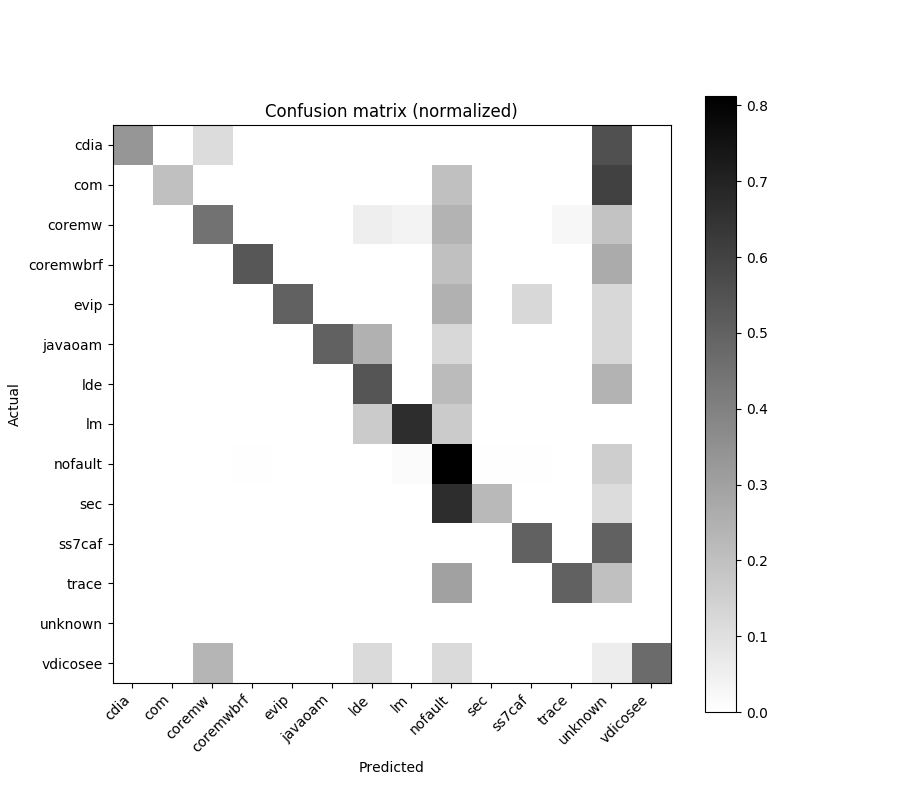
\includegraphics[width=\textwidth]{results/figures/256_32_10pcterror.png}
    \caption{The confusion matrix of the classification made by the HTM model with ten per cent word drop-out in each sequence. The vertical axis represent the actual sequence presented to the HTM model, and the horizontal axis represent the predicted fault class.}
    \label{fig:10confmatrix}
\end{figure}
\raggedbottom

\begin{figure}[H]
  \centering
    \scalebox{.61}{    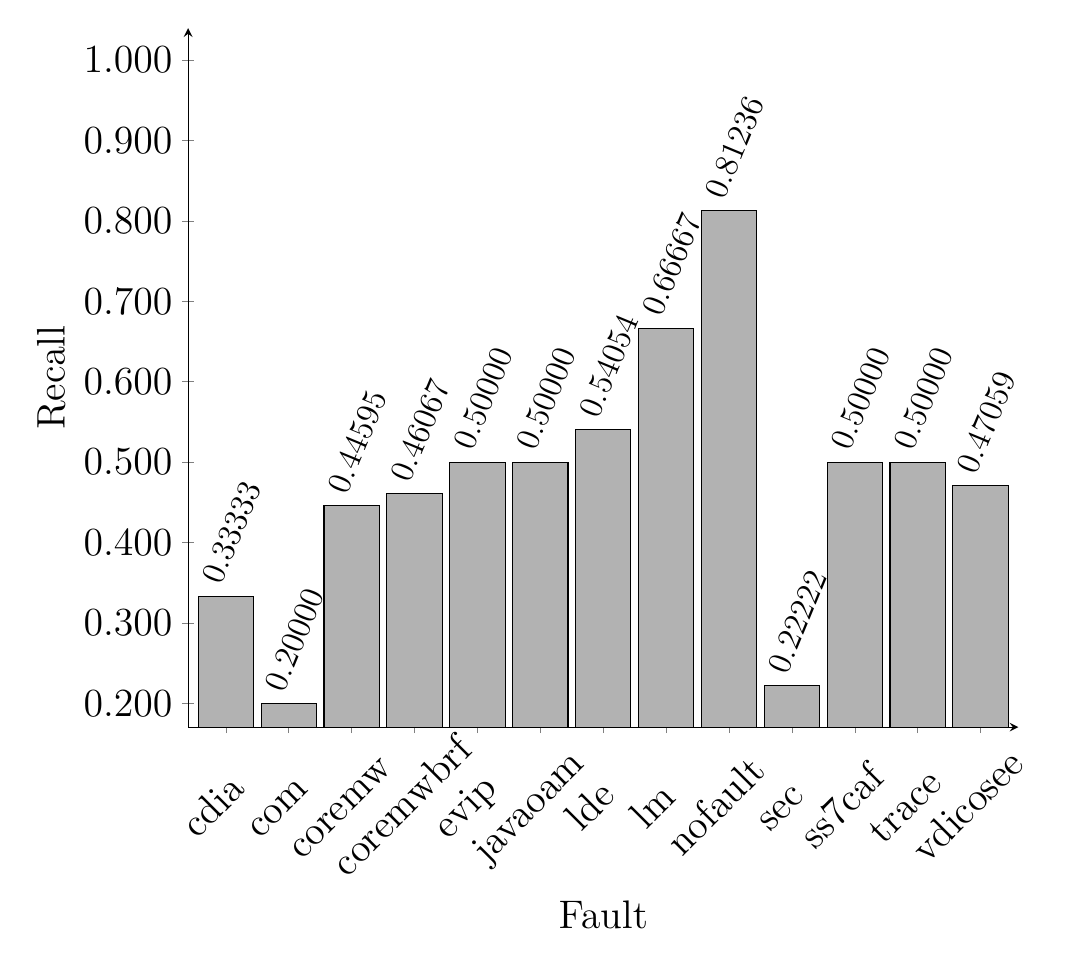
\begin{tikzpicture}[font=\Large]
    \begin{axis}[
      width=\textwidth,
      ybar,
      font=\Large,
      bar width=20pt,
      xlabel={Fault},
      ylabel={Recall},
      xticklabel style={rotate=45,anchor=base,yshift=-20,xshift=-22},
      xtick=data,
      ymin=0.2100,
      ymax=1.00,
      axis x line=bottom,
      axis y line=left,
      enlarge x limits=0.1,
      enlargelimits=0.05,
      domain=0.21:1.000,
              y tick label style={
            /pgf/number format/.cd,
            fixed,
            zerofill,
            precision=3,
            /tikz/.cd,},
      symbolic x coords={cdia,com,coremw,coremwbrf,evip,javaoam,lde,lm,nofault,sec,ss7caf,trace,vdicosee},
      nodes near coords={\pgfmathprintnumber[fixed zerofill, precision=5]{\pgfplotspointmeta}},
      every node near coord/.append style={color=black, rotate=67.5, anchor=center, font=\large, xshift=22, yshift=7}],

    ]
      \addplot[fill=black!30] coordinates {
        (cdia,0.33333) (com,0.2) 
		(coremw,.445946) (coremwbrf,0.460674) (evip,0.5) (javaoam, 0.5) (lde, 0.540541) (lm, 0.666667) (nofault,0.812364) (sec, 0.222222) (ss7caf, .5) (trace, 0.5) (vdicosee,0.470588)
      };
    \end{axis}
  \end{tikzpicture}}
    \caption{Recall of each fault class, with ten per cent word drop-out of each sequence.}
    \label{fig:recall10}

    \vspace*{\floatsep}

    \scalebox{.61}{    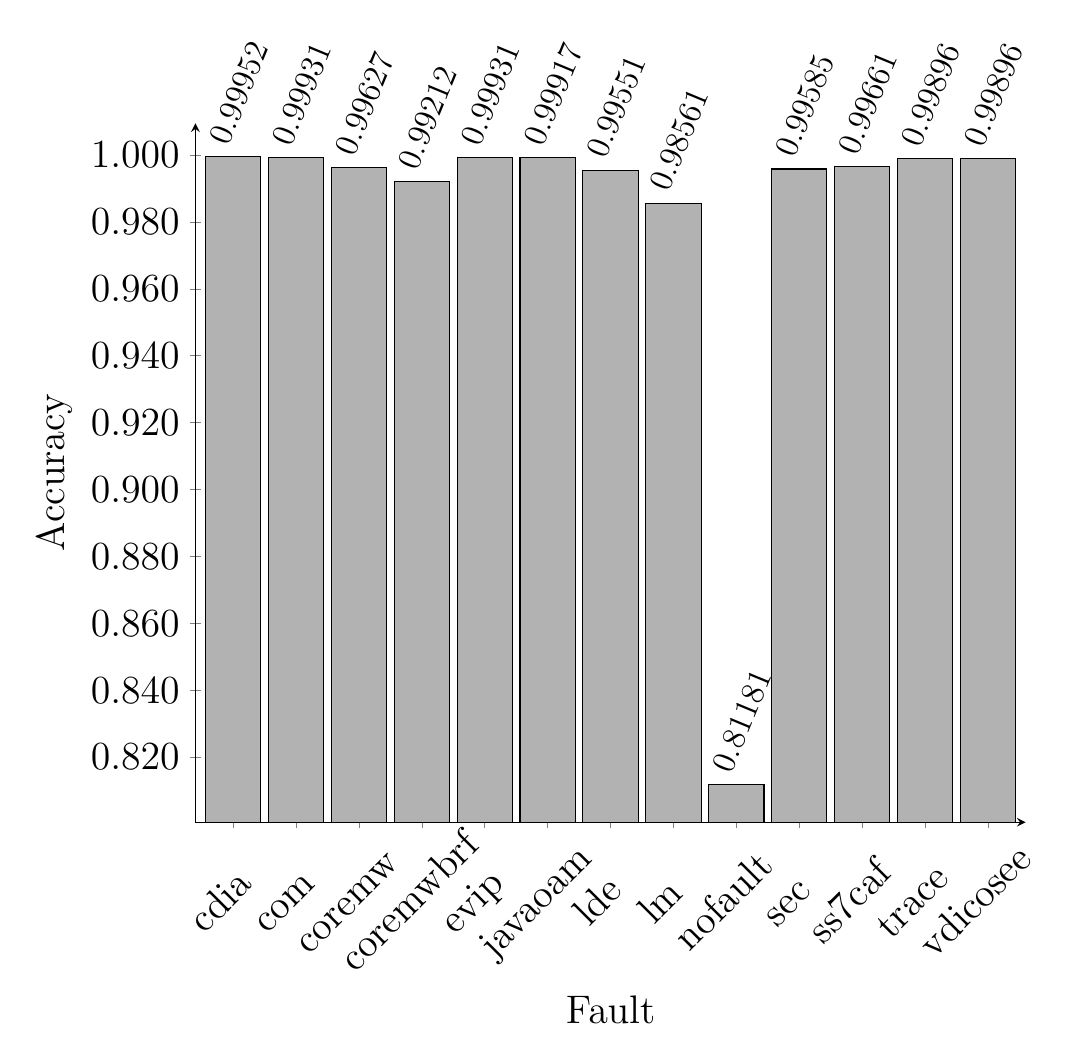
\begin{tikzpicture}[font=\Large]
    \begin{axis}[
      width=\textwidth,
      ybar,
      font=\Large,
      bar width=20pt,
      xlabel={Fault},
      ylabel={Accuracy},
      xticklabel style={rotate=45,anchor=base,yshift=-20,xshift=-22},
      xtick=data,
      ymin=0.81000,
      ymax=1.000000,
      axis x line=bottom,
      axis y line=left,
      enlarge x limits=0.1,
      enlargelimits=0.05,
      domain=0.800:1.000000,
              y tick label style={
            /pgf/number format/.cd,
            fixed,
            zerofill,
            precision=3,
            /tikz/.cd,},
      symbolic x coords={cdia,com,coremw,coremwbrf,evip,javaoam,lde,lm,nofault,sec,ss7caf,trace,vdicosee},
      nodes near coords={\pgfmathprintnumber[fixed zerofill, precision=5]{\pgfplotspointmeta}},
      every node near coord/.append style={color=black, rotate=67.5, anchor=center, font=\large, xshift=22, yshift=7}],

    ]
      \addplot[fill=black!30] coordinates {
        (cdia,0.999516) (com,0.999308) 
		(coremw,.996265) (coremwbrf,0.992116) (evip,0.999308) (javaoam, 0.99917) (lde, 0.995505) (lm, 0.985614) (nofault,0.811813) (sec, 0.99585) (ss7caf, .996611) (trace, 0.998963) (vdicosee,0.998963)
      };
    \end{axis}
  \end{tikzpicture}}
    \caption{Classification accuracy of each fault class, with ten per cent word drop-out of each sequence.}
    \label{fig:acc10}
\end{figure}



\subsection{Inference With 20 Per Cent Drop-Out}
The trend from the previous experiment is continuing with a drop-out of twenty per cent. The pattern in the confusion matrix, \autoref{fig:20confmatrix}, is starting to appear random, which means the HTM model has trouble labelling any class correctly in the majority of cases. However, the fault class \textit{ss7caf} is correctly classified in all cases, but from \autoref{table:dataset} we can see that \textit{ss7caf} only contain two examples. Thus, no real conclusions can be drawn from this, especially since \autoref{fig:recall10} shows that it misclassified \textit{ss7caf} 50 per cent of the time. The severity of the decline is also evident in \autoref{fig:recall20}, with HTM model having a recall of around 20-30 per cent. In \autoref{fig:acc20}, the accuracy is still saturated for all classes except \textit{nofault}, which has now dropped to $59.167$ per cent. 

\begin{figure}[H]
%    \vspace{-.2cm}
    \centering
    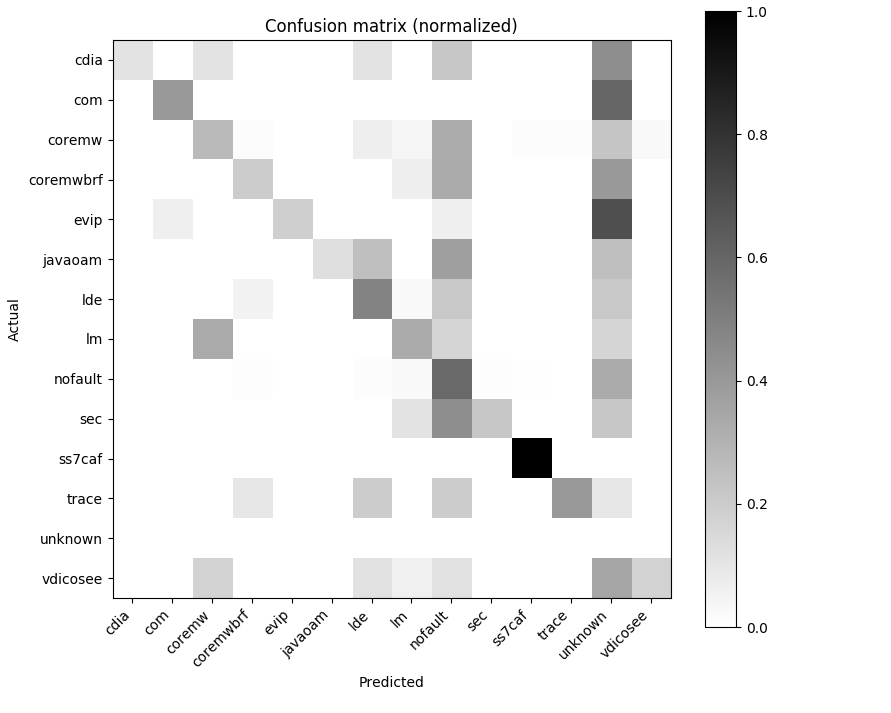
\includegraphics[width=\textwidth]{results/figures/256_32_20pcterror_v2.png}
    \vspace{-1cm}
    \caption{The confusion matrix of the classification with twenty per cent word drop-out. The vertical axis represent the actual sequence label presented, and the horizontal axis represent the predicted fault label.}
    \label{fig:20confmatrix}
\end{figure}

\raggedbottom



\begin{figure}[H]
  \centering
    \scalebox{.61}{    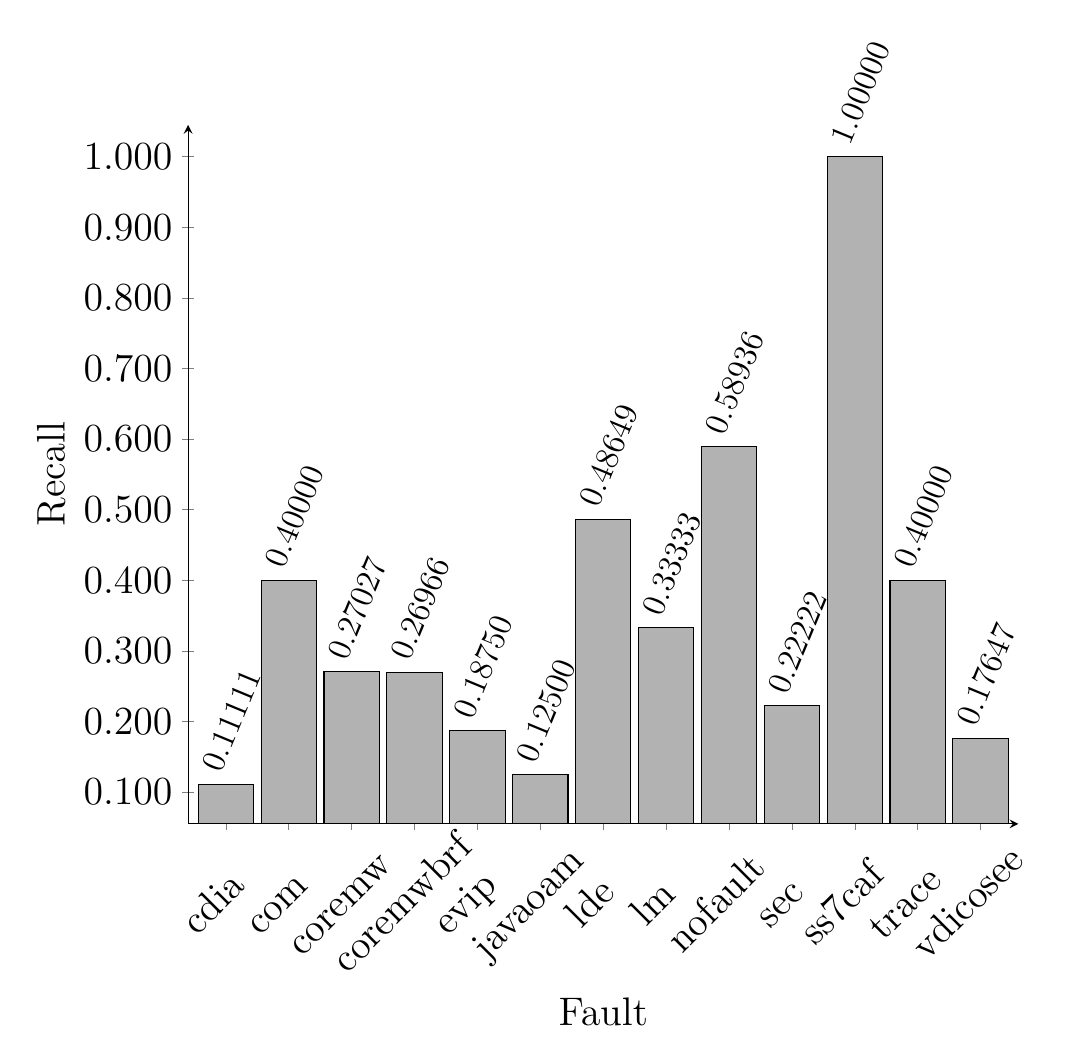
\begin{tikzpicture}[font=\Large]
    \begin{axis}[
      width=\textwidth,
      ybar,
      font=\Large,
      bar width=20pt,
      xlabel={Fault},
      ylabel={Recall},
      xticklabel style={rotate=45,anchor=base,yshift=-20,xshift=-22},
      xtick=data,
      ymin=0.100,
      ymax=1.00,
      axis x line=bottom,
      axis y line=left,
      enlarge x limits=0.1,
      enlargelimits=0.05,
      domain=0.10:1.000,
              y tick label style={
            /pgf/number format/.cd,
            fixed,
            zerofill,
            precision=3,
            /tikz/.cd,},
      symbolic x coords={cdia,com,coremw,coremwbrf,evip,javaoam,lde,lm,nofault,sec,ss7caf,trace,vdicosee},
      nodes near coords={\pgfmathprintnumber[fixed zerofill, precision=5]{\pgfplotspointmeta}},
      every node near coord/.append style={color=black, rotate=67.5, anchor=center, font=\large,  xshift=22, yshift=7}],

    ]
      \addplot[fill=black!30] coordinates {
        (cdia,0.11111) (com,0.4) 
		(coremw,.27027) (coremwbrf,0.269663) (evip,0.1875) (javaoam, 0.125) (lde, 0.486486) (lm, 0.333333) (nofault,0.589362) (sec, 0.222222) (ss7caf, 1.0) (trace, 0.4) (vdicosee,0.176471)
      };
    \end{axis}
  \end{tikzpicture}}
    \caption{Recall of each fault class, with twenty per cent word drop-out of each sequence.}
    \label{fig:recall20}

    \vspace*{\floatsep}

    \scalebox{.61}{    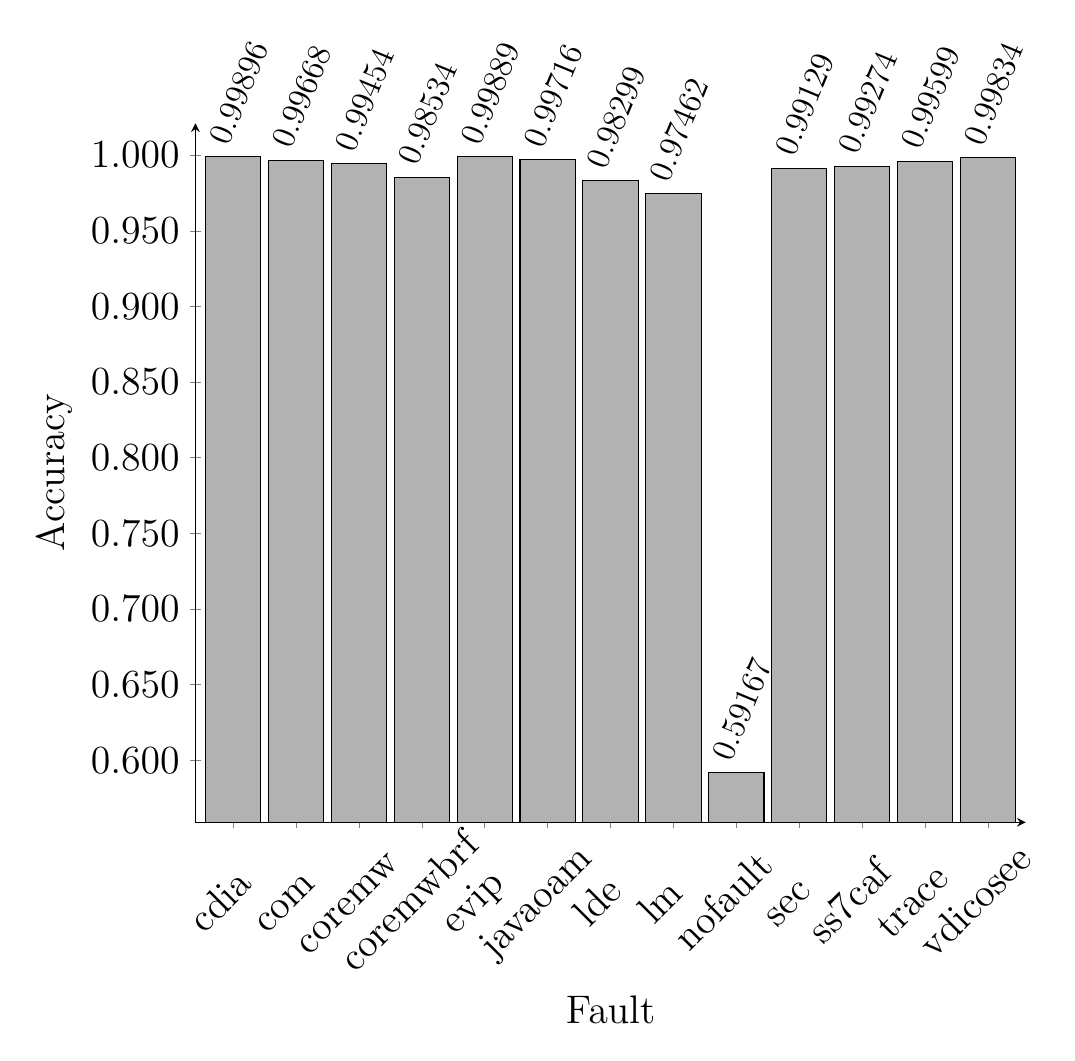
\begin{tikzpicture}[font=\Large]
    \begin{axis}[
      width=\textwidth,
      ybar,
      font=\Large,
      bar width=20pt,
      xlabel={Fault},
      ylabel={Accuracy},
      xticklabel style={rotate=45,anchor=base,yshift=-20,xshift=-22},
      xtick=data,
      ymin=0.58000,
      ymax=1.000000,
      axis x line=bottom,
      axis y line=left,
      enlarge x limits=0.1,
      enlargelimits=0.05,
      domain=0.5800:1.000000,
              y tick label style={
            /pgf/number format/.cd,
            fixed,
            zerofill,
            precision=3,
            /tikz/.cd,},
      symbolic x coords={cdia,com,coremw,coremwbrf,evip,javaoam,lde,lm,nofault,sec,ss7caf,trace,vdicosee},
      nodes near coords={\pgfmathprintnumber[fixed zerofill, precision=5]{\pgfplotspointmeta}},
      every node near coord/.append style={color=black, rotate=67.5, anchor=center, font=\large, xshift=22, yshift=7}],

    ]
      \addplot[fill=black!30] coordinates {
        (cdia,0.998963) (com,0.99668) 
		(coremw,.994536) (coremwbrf,0.985338) (evip,0.998893) (javaoam, 0.997164) (lde, 0.982986) (lm, 0.974618) (nofault,0.591673) (sec, 0.991286) (ss7caf, .992738) (trace, 0.995989) (vdicosee,0.99834)
      };
    \end{axis}
  \end{tikzpicture}}
    \caption{Classification accuracy of each fault class, with twenty per cent word drop-out of each sequence.}
    \label{fig:acc20}
\end{figure}



\subsection{Comparison With Linnaeus}
The final evaluation is a comparison with the already existing classifier \textit{Linnaeus}. If the HTM model should be an viable option in a production setting, it should have comparable or better statistics than \textit{Linnaeus}. However, the machine learning models where benchmarked on different computers, thus contributing to the differences in the timing reports.

The \textit{Linnaeus} model was benchmarked on a computer with an Intel(R) Xenon(R) CPU ES-2658 v2 processor with 40 cores, Skylake microarchitecture, and 2.4 GHz clock frequency. During training 20 cores are utilised at 100 per cent. The HTM model was benchmarked on a computer with an Intel i5-6300U processor with two cores, and with clock frequency of 2.4 GHz. During training and testing of the HTM model one core was utilised at 100 per cent.


In \autoref{tab:stats}, the comparable statistics are presented. We start by introducing the statistics for the \textit{Linnaeus} model. The first two model types are \textit{word n-grams}, where $n$ contiguous words in each system log are bagged together to form a vocabulary. The next two models are \textit{character n-grams}, and instead of words, $n$ contiguous characters are bagged together. Vocabulary build time represents the time it takes to build the different vocabularies based on the model chosen. The total training time is therefore sum of vocabulary build time and training time. The service side is the occupied memory usage when classifying new system logs. The classification latency represents the time it takes to classify a part of a system log file at a time, currently 88 kB at a time. The test accuracy is based on unseen portion of the data set, i.e. the training and testing set were separated. As shown in \autoref{tab:stats}, the accuracy for the models is obtain through several runs where training and testing are split different each time. The accuracy range from $70-95$ per cent for the different models using the test set, and $98-100$ per cent during training.



\begin{table}[H]
\centering
\renewcommand\arraystretch{1.2}
\tiny

\caption{The comparable statistics between the two machine learning models.}
\label{tab:stats}

\begin{tabularx}{\textwidth}{@{} ccccccc}
    \toprule
    &&& &&&\\
    &&\multicolumn{3}{c}{\centering\parbox{5cm}{\centering\large\textbf{Linnaeus Model}}} \\
    &&& &&&\\
    \multirow{2}{*}{\centering\parbox{1.5cm}{\centering \\Configuration}} & \multirow{2}{*}{\centering\parbox{1cm}{\centering Train\\Accuracy}}  & \multirow{2}{*}{\centering\parbox{1cm}{\centering Test\\Accuracy}} & \multirow{2}{*}{\centering\parbox{1.5cm}{\centering Vocabulary\\Build Time}} & \multirow{2}{*}{\centering\parbox{1cm}{\centering Training\\Time}} & \multirow{2}{*}{\centering\parbox{1cm}{\centering Service\\Size}} & \multirow{2}{*}{\centering\parbox{1.5cm}{\centering Classification\\Latency}}\\
    &&&&&&\\
    \midrule
            Word ngrams = 1 & $99\%$ & $75-95\%$ & 42 s &150 s& 150 MiB & 10 ms\\
            Word ngrams = 2 & $98\%$ & $75-95\%$ & 109 s &217 s & 150 MiB & 17 ms\\
            Char ngrams = 2 & $100\%$ & $70-95\%$ & 787 s &787 s & 150 MiB & 68 ms\\
            Char ngrams = 4 & $99\%$ & $70-95\%$ & 514 s &514 s& 150 MiB & 42 ms\\
    \bottomrule
\end{tabularx}


\begin{tabularx}{\textwidth}{@{} ccccccc}
    &&& &&&\\
    \multicolumn{6}{c}{\centering\parbox{5cm}{\centering\large\textbf{HTM Model}}} \\
    &&& &&&\\
    \multirow{2}{*}{\centering\parbox{2cm}{\centering \\Experiment}}    & \multirow{2}{*}{\centering\parbox{2cm}{\centering Train\\Accuracy}}   &\multirow{2}{*}{\centering\parbox{1.5cm}{\centering Build\\Time}} &\multirow{2}{*}{\centering\parbox{2cm}{\centering Training\\Time}} & \multirow{2}{*}{\centering\parbox{1cm}{\centering Service\\Size}}&\multirow{2}{*}{\centering\parbox{2cm}{\centering Classification\\Latency}}&\\
    &&& &&&\\
    \midrule
    $0\%$ drop-out & $98.6\%$      &131 s      &828 s        &888 MiB     &88 ms&\\
    $10\%$ drop-out& $80.7\%$     &--        &--         &888 MiB     &88 ms&\\
    $20\%$ drop-out& $58.5\%$      &--        &--          &888 MiB     &88 ms&\\
    \bottomrule
\end{tabularx}
\end{table}


Let us now introduce the statistics of the HTM model, also presented in \autoref{tab:stats}. Instead of model configurations, we present the accuracy obtained from the model during the three experiments performed. We can see a clear degradation of the accuracy as we introduce faults into the system log sequences, from 98.6 to 58.5 per cent. The reason we preformed this test is to see how well the HTM model preformed with added errors to the sequences. This test is however not really comparable to the \textit{Linnaeus} models, but it does tell us how well it is at classifying incomplete system logs. Next, we have the build time, which is the time it takes to perform all the preprocessing steps required. The training time represent the time it took to train the HTM model using \textit{one-shot learning}. Service size is the memory usage of the HTM model. An important thing to note is that the most of the memory usage is due to the allocation lists used for encoding, decoding, and the entire system log data set. The network size is only 178 MiB of the entire 888 MiB. Classification latency is the time it takes to encode each word to an SDR, present it to the HTM model, and decode a prediction at the end of a system log sequence. 


From comparing the statistics, the \textit{Linnaeus} models achieves similar results in the training cases as the HTM model. The classification of the system logs are performed in different ways, where the \textit{Linnaeus} model takes system log chunks and processes them, where as the HTM model looks at individual logs, one at a time. It is likely that the execution time for all parts of the HTM model would be faster if it where evaluated on a better machine. But with current metrics, the \textit{Linnaeus} model has the benefit have lower classification latency and smaller memory footprint, i.e. service size.

The test with 10 and 20 per cent dropout with HTM model is interesting, as they give some indication on how well the model is at being able to classifying system logs if the vocabulary is changed. However, with the current HTM model we can see that it does not adapt well to introduced errors in the system log sequences. 



%176MB Network size